\chapter{Surface (Triangle mesh)}
\label{cap_surface}

At InVesalius, a 3D surface is generated based on a image segmentation. A surface is generated using the \textit{marching cubes} algorithm. In a nutshell, this algorithm transforms \textit{voxels} from the stacked and segmented images to polygons (triangles in this case).

On the left panel, inside \textbf{3. Configure 3D surface}, \textbf{Surface properties} you have the controls to configure a 3D surface.

\begin{figure}[!htb]
\centering
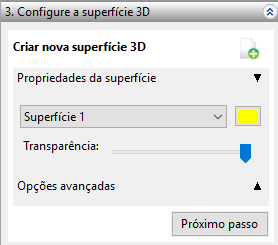
\includegraphics[scale=0.65]{surface_config_panel_pt.png}
\caption{3D surface configuration.}
\label{fig:3d_surface_managment}
\end{figure}


\section{Creating 3D surfaces}

It's possible create a new surface based on a already segmented mask. To do that, on the left panel, \textbf{3. Configure 3D surface}, click on the button shown at the figure~\ref{fig:shortcut_new_surface}.

\begin{figure}[!htb]
\centering

\includegraphics[scale=0.18]{object_add_original}
\caption{Button to create a 3D surface.}
\label{fig:shortcut_new_surface}
\end{figure}

After clicking this button a dialog will be shown (figure \ref{fig:create_surface_1}). This dialog allows to configure the 3D surface creation. It allows to set the quality of the surface, to fill the surface holes and to keep only the largest connected region of the surface.

\begin{figure}[!htb]
\centering
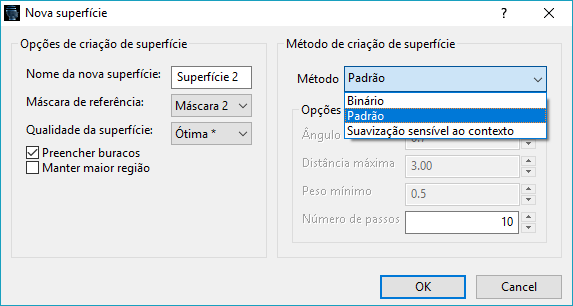
\includegraphics[scale=0.5]{surface_config_window_pt.png}
\caption{3D surface creation dialog.}
\label{fig:create_surface_1}
\end{figure}

%Existe 2 opções para fechar os buracos existentes e para selecionar a maior região da superfície aonde em muitos
%casos é útil para remover o suporte ou a mesa do tomografo.

The keep largest region option may be used, for instance, to remove the tomograph support. Figure~\ref{fig:surface_ex1} displays a surface created with \textbf{Keep largest region} and \textbf{Fill holes} activated. 

\begin{figure}[!htb]
  \centering
  \subfloat[Frente]{\label{fig:__1}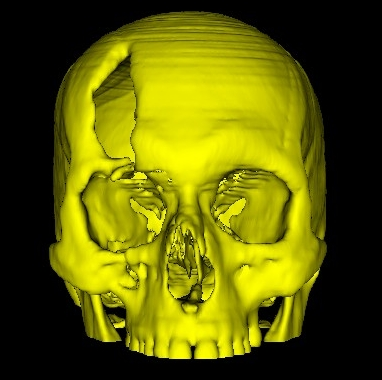
\includegraphics[width=0.338\textwidth]{surface_model_front.jpg}}
  \subfloat[Baixo]{\label{fig:__1}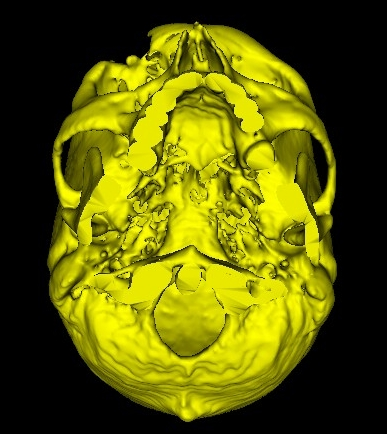
\includegraphics[width=0.3\textwidth]{surface_model_bottom.jpg}}
  \caption{Surface created with the options \textbf{Keep largest region} and \textbf{Fill holes} activated.}
  \label{fig:surface_ex1}
\end{figure}

Whereas the figure~\ref{fig:surface_ex2} displays the surface create without activating that options. Note the tomograph support and the holes.

\begin{figure}
  \centering
  \subfloat[Frente]{\label{fig:__2}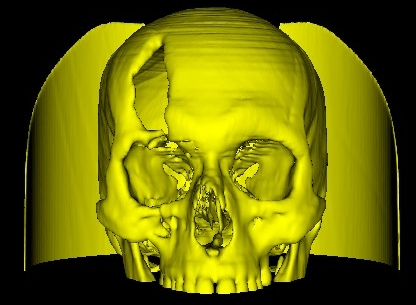
\includegraphics[width=0.371\textwidth]{surface_model_front_all_parts.jpg}}
  \subfloat[Baixo]{\label{fig:__2}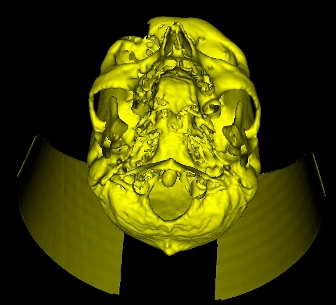
\includegraphics[width=0.3\textwidth]{surface_model_bottom_all_parts.jpg}}
  \caption{Surface created with the options \textbf{Keep largest region} and \textbf{Fill holes} deactivated.}
  \label{fig:surface_ex2}
\end{figure}

The item \textbf{Surface creation method} has the following options:\textbf{Binary}, \textbf{Context aware smoothing} and \textbf{Default}. Figure~\ref{fig:surf_method} shows an example of surface created using each of these 3 methods.

O método \textbf{binário}, tem como partida a máscara que foi segmentada, sendo a região selecionada como 1 e o restante 0. Como existem somente 2 valores, as curvas na superfície que o algoritmo gera são abruptas ou popularmente conhecida como "degraus".

The \textbf{Binary} method takes as input the segmentation mask which is binary, where selected regions have value 1 and non-selected have value 0. As it is binary, the surface generated has a blocky aspect, mainly in high curvature areas.

No método \textbf{Context aware smoothing}, inicialmente a superfície é gerada a partir do método binário, mas em seguida é executado o algoritmo "Context aware smoothing" para suavizar a superfície resultante e evitar os "degraus" na mesma. Neste passo é requerido 4 valores, que serão apresentados a seguir.

O \textbf{ângulo}, nesse caso será formado entre 2 normais de triângulos adjacentes, que \textbf{caso esteja acima do valor} definido no campo ângulo, o triângulo é elegido para ser o ponto de partida da suavização, a faixa de valor é de 0 até 1, sendo $0^\circ$ e $90^\circ$ respectivamente. A \textbf{distância máxima} é o raio a partir dos triângulos elegidos no passo anterior, que será utilizada como limite de suavização. O \textbf{peso mínimo} é o quanto de suavização será aplicado nas áreas que estão fora do raio determinado anteriormente. O \textbf{número de passos} é quantas vezes o algoritmo vai executar.

O método \textbf{padrão} é ativo \textbf{somente quando não existir edição manual na máscara}, os pixeis da imagem original que estão sob a máscara é utilizado para a geração de superfície, como normalmente imagens de tomografia ou ressonância possui vários níveis de cinza, é gerada uma superfície com curvas mais suaves.

\begin{figure}[!htb]
  \centering
  \subfloat[Binário]{\label{fig:surf_binary}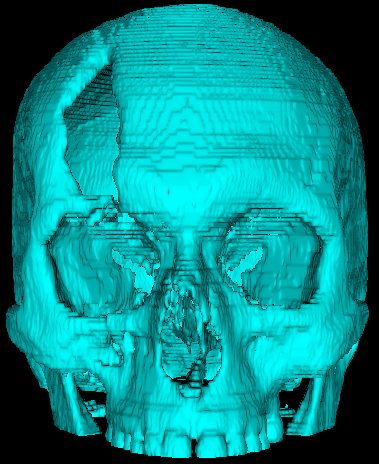
\includegraphics[width=0.33\textwidth]{binary.png}}
  \hfill
  \subfloat[Context aware]{\label{fig:surf_context}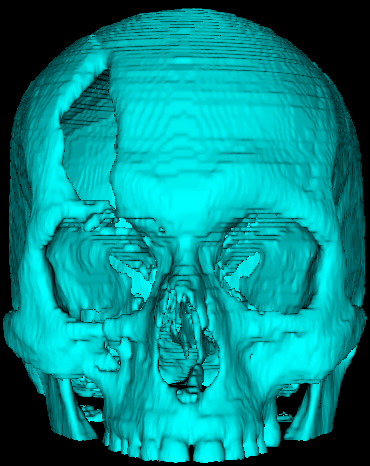
\includegraphics[width=0.32\textwidth]{context.png}}
  \hfill
  \subfloat[Padrão]{\label{fig:surfa_default}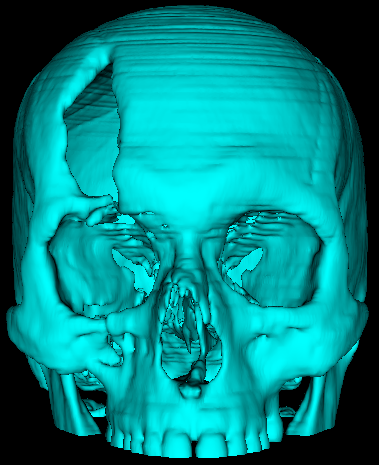
\includegraphics[width=0.332\textwidth]{default.png}}
  \caption{Superfícies geradas por diferentes métodos }
  \label{fig:surf_method}
\end{figure}



\section{Transparência}

É possível visualizar uma superfície com transparência. Para isso, primeiro selecione a
superfície por meio da lista de seleção, dentro do item \textbf{3. Configure a superfície 3D}, opção
\textbf{Propriedades da superfície} (figure \ref{fig:select_surface}).

\begin{figure}[!htb]
\centering
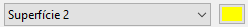
\includegraphics[scale=0.8]{surface_select_menu.png}
\caption{Seleção de superfície}
\label{fig:select_surface}
\end{figure}

Em seguida, para determinar o nível de transparência que a superfície selecionada receberá, arraste
o controle deslizante ilustrado na figure \ref{fig:select_transparency}. Quanto mais para a direita
o controle, maior será a transparência aplicada.

\begin{figure}[!htb]
\centering
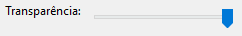
\includegraphics[scale=0.7]{surface_transparency_pt.png}
\caption{Seleção de nível de transparência}
\label{fig:select_transparency}
\end{figure}

A figure \ref{fig:model_transparency} ilustra a visualização de duas superfícies: uma mais externa
(esverdeada) e outra mais interna (amarelada). A superfície mais externa aparece com a transparência
aumentada.

\begin{figure}[!htb]
\centering
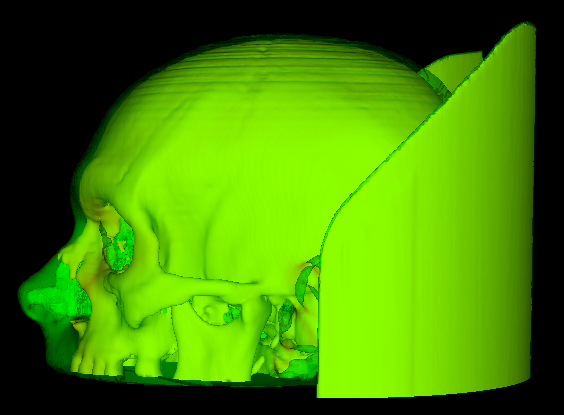
\includegraphics[scale=0.3]{transparency_2}
\caption{Superfícies com nível alterado de transparência}
\label{fig:model_transparency}
\end{figure}

\newpage

\section{Cor}

A cor de uma superfície também pode ser alterada. Selecione a superfície (reveja a figure
\ref{fig:select_surface}) e, em seguida, clique no botão ao lado da superfície selecionada. A figure
\ref{fig:change_surface_color} ilustra o botão, também localizado no item \textbf{3. Configure a
superfície 3D}, opção \textbf{Propriedades da superfície}.

\begin{figure}[!htb]
\centering
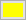
\includegraphics[scale=0.6]{surface_button_select_color_yellow.png}
\caption{Botão para alteração de cor}
\label{fig:change_surface_color}
\end{figure}

Uma janela de seleção de cores se abre (figure \ref{fig:button_select_color}). Selecione a cor
desejada e clique no botão \textbf{OK}.

\begin{figure}[!htb]
\centering
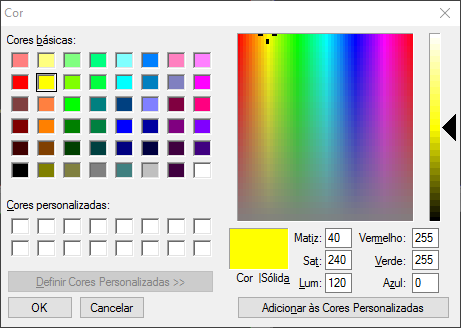
\includegraphics[scale=0.6]{surface_select_color_windows_so_pt.png}
\caption{Opções de cor}
\label{fig:button_select_color}
\end{figure}

\section{Separando regiões desconexas}

Para separar regiões da superfície que se encontram desconexas, é necessário clicar na opção
\textbf{Ferramentas avançadas}, dentro do item \textbf{3. Configure a superfície 3D}. Veja a
figure \ref{fig:advanced_tools}.

\begin{figure}[!htb]
\centering
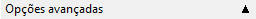
\includegraphics[scale=0.7]{surface_painel_advanced_options_pt.png}
\caption{Atalho para opções avançadas}
\label{fig:advanced_tools}
\end{figure}

\newpage

Um menu com as opções disponíveis será exibido, como ilustra a figure
\ref{fig:advanced_tools_expanded}.

\begin{figure}[!htb]
\centering
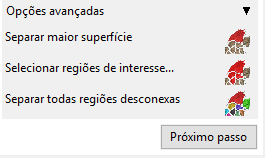
\includegraphics[scale=0.7]{surface_split_pt.png}
\caption{Opções avançadas}
\label{fig:advanced_tools_expanded}
\end{figure}

\subsection{Separar maior superfície}

A opção \textbf{Separar maior superfície} seleciona, automaticamente, somente a região
desconexa que contém maior volume. Para realizar a operação, basta clicar no atalho
que a figure \ref{fig:short_connectivity_largest} ilustra. É criada uma nova superfície
resultante da operação.

\begin{figure}[!htb]
\centering
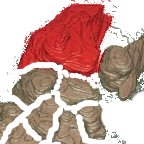
\includegraphics[scale=0.2]{connectivity_largest}
\caption{Atalho para separação da maior região desconexa}
\label{fig:short_connectivity_largest}
\end{figure}

Como exemplo, a figure \ref{fig:extract_most_region_1} mostra um caso antes da separação
da maior região.

\begin{figure}[!htb]
\centering
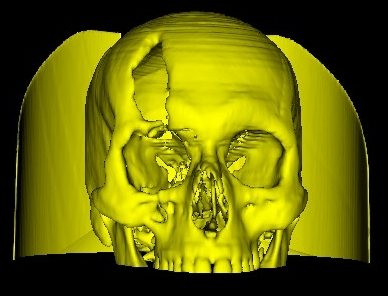
\includegraphics[scale=0.3]{surface_extract_most_region_1.jpg}
\caption{Superfícies desconexas}
\label{fig:extract_most_region_1}
\end{figure}

Na figure \ref{fig:extract_most_region2}, observa-se a superfície com a maior região
desconexa separada.

\begin{figure}[!htb]
\centering
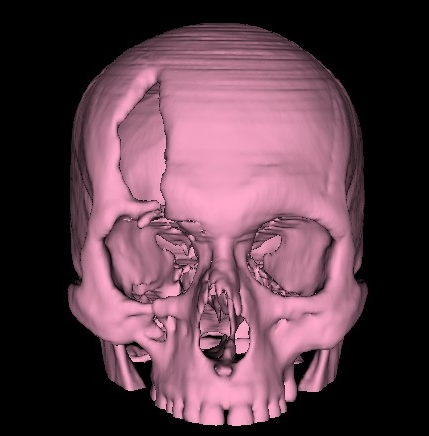
\includegraphics[scale=0.3]{surface_extract_most_region2.jpg}
\caption{Maior região separada}
\label{fig:extract_most_region2}
\end{figure}

\newpage

\subsection{Selecionar as regiões de interesse}

Outra modalidade de seleção se dá pela opção \textbf{Selecionar as regiões de interesse...}.
Para ativá-la, o usuário deve clicar sobre o botão ilustrado na figure
\ref{fig:short_connectivity_manual}. Em seguida, basta clicar sobre as regiões desconexas
da superfície que se pretende selecionar.

\begin{figure}[!htb]
\centering
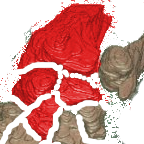
\includegraphics[scale=0.2]{connectivity_manual}
\caption{Atalho para seleção de regiões de interesse}
\label{fig:short_connectivity_manual}
\end{figure}

No exemplo da figure \ref{fig:extract_most_region3}, foram selecionados o crânio e a parte
direita do suporte do tomógrafo.

\begin{figure}[!htb]
\centering
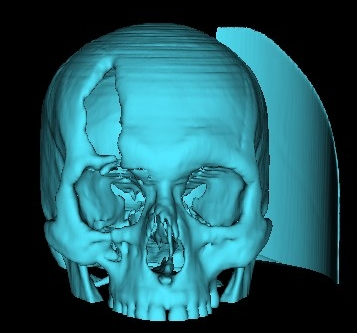
\includegraphics[scale=0.35]{surface_extract_most_region3.jpg}
\caption{Exemplo de regiões de interesse selecionadas}
\label{fig:extract_most_region3}
\end{figure}


\subsection{Separar todas regiões desconexas}

É possível, também, separar automaticamente \textit{todas} as regiões desconexas. Para
isso, basta clicar no botão ilustrado pela figure \ref{fig:connectivity_split_all}, que
representa a opção \textbf{Separar todas regiões desconexas}.

\begin{figure}[!htb]
\centering
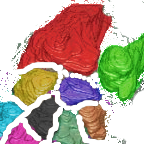
\includegraphics[scale=0.2]{connectivity_split_all}
\caption{Atalho para separação de todas as regiões desconexas}
\label{fig:connectivity_split_all}
\end{figure}

A figure \ref{fig:extrac_most_region_4} mostra um exemplo.

\begin{figure}[!htb]
\centering
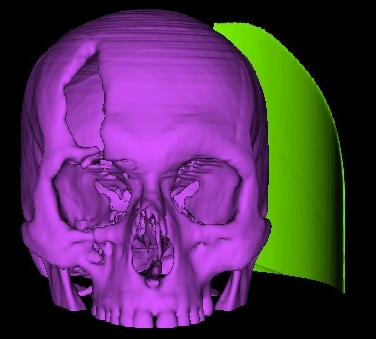
\includegraphics[scale=0.3]{surface_extract_most_region_4.jpg}
\caption{Exemplo de separação de todas as regiões desconexas}
\label{fig:extrac_most_region_4}
\end{figure}

